\chapter{Experiment and Result}
brief of experiment and result.
\section{Experiment}
Please tell how the experiment conducted from method.

\section{Result}
Please provide the result of experiment

\section{Lusia Violita Aprilian/1164080}

\subsection{Teori}
\begin{enumerate}
\item Klasifikasi teks
	\par Klasifikasi Dokumen / Teks adalah salah satu tugas penting dan tipikal dalam supervised machine learning (ML). Menetapkan kategori pada dokumen, yang dapat berupa halaman web, buku perpustakaan, artikel media, galeri, dll. Memiliki banyak aplikasi seperti mis. penyaringan spam, perutean email, analisis sentimen dll. 
	\begin{figure}[ht]
		\centering
		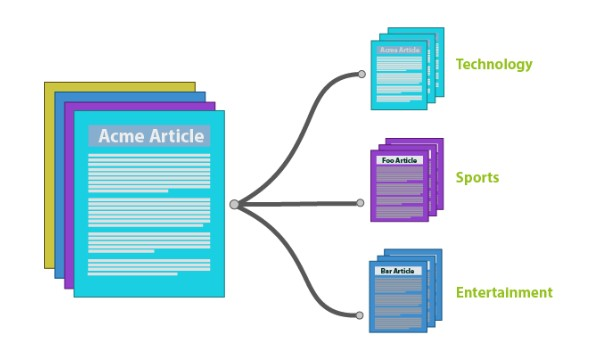
\includegraphics[scale=0.5]{figures/m1.jpg}
		\caption{Lusia-Klasifikasi teks}
		\label{contoh}
	\end{figure}
	
\item Klasifikasi Bunga tidak dapat penggunakan machine learning
	\par Klasifikasi bunga tidak dapat menggunakan machine learning karena memiliki masalah input yang serupa namun output yang berbeda atau 'noise'. Yang dimaksud dengan noise adalah contoh output yang direkam bukan seperti seharusnya. Misalnya saja kita secara implisit berasumsi bahwa contoh bunga kita telah diklasifikasikan dengan benar. Tetapi ini harus dilakukan dengan seseorang yang tepat, seperti seorang ahli botani. Seorang ahli botani ahli harus melihat contoh bunga dan berkata: " ini adalah setosa ... ini adalah virginica ", dan dengan demikian bertindak sebagai "guru" yang memungkinkan mesin untuk belajar. Tetapi bagaimana jika guru itu melakukan kesalahan? Selain itu, selalu ada peluang untuk memperkenalkan kesalahan saat merekam data. Noise juga ditemukan dalam pengukuran, yang selalu sedikit bermasalah karena alat dan sensor kami tidak sempurna dan hanya bekerja pada tingkat presisi tertentu.
	\begin{figure}[ht]
		\centering
		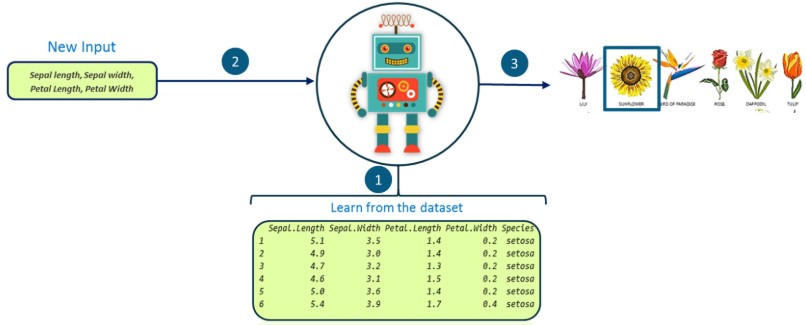
\includegraphics[scale=0.5]{figures/m2.jpg}
		\caption{Lusia-Klasifikasi bunga}
		\label{contoh}
	\end{figure}

\item Teknik pembelajaran mesin pada teks YouTube
	\par Dengan menggunakan kasus seperti rekomendasi video yang terdapat pada fiturnya, Machine Learning pada YouTube memperhatikan apa saja yang menarik perhatian para penggunanya. Ketika kita sedang menonton di YouTube, pada sebelah kanan terdapat 'Up Next' yang menampilkan beberapa video serupa yang sedang ditonton. Dan ketika mengklik salah satu video dari baris tersebut, maka YouTube akan mengingatnya dan menggunakan kata yang tertera sebagai referensi. 
	\begin{figure}[ht]
		\centering
		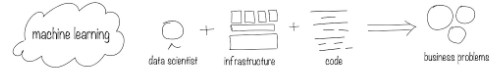
\includegraphics[scale=0.5]{figures/m3.jpg}
		\caption{Lusia-Teknik YouTube}
		\label{contoh}
	\end{figure}

\item Vectorisasi Data
	\begin{itemize}
		\item Maksud dari Vectorisasi Data merupakan Pemecahan dan Pembagian Data.
	\end{itemize}
	
\item Bag of word
	\par Bag-of-words adalah cara untuk merepresentasikan data teks saat memodelkan teks dengan algoritma pembelajaran mesin.
	\begin{figure}[ht]
		\centering
		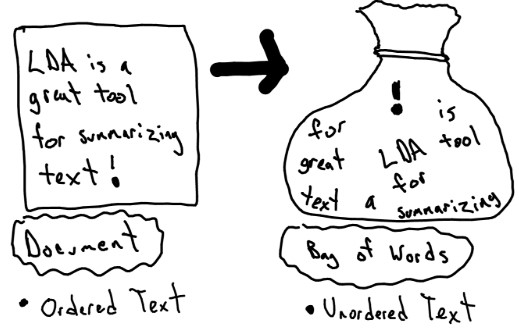
\includegraphics[scale=0.5]{figures/m5.jpg}
		\caption{Lusia-Bag of Word}
		\label{contoh}
	\end{figure}
	
\item TF-IDF
	\par TF-IDF merupakan istilah frekuensi - frekuensi dokumen terbalik, adalah ukuran penilaian yang banyak digunakan dalam pengambilan informasi (IR) atau peringkasan. TF-IDF dimaksudkan untuk mencerminkan seberapa relevan suatu istilah dalam dokumen yang diberikan. Intuisi di baliknya adalah bahwa jika sebuah kata muncul beberapa kali dalam sebuah dokumen, kita harus meningkatkan relevansinya karena itu harus lebih bermakna daripada kata-kata lain yang muncul lebih sedikit kali (TF). Pada saat yang sama, jika sebuah kata muncul berkali-kali dalam suatu dokumen tetapi juga di sepanjang banyak dokumen lain, mungkin itu karena kata ini hanya kata yang sering; bukan karena itu relevan atau bermakna (IDF).
	\begin{figure}[ht]
		\centering
		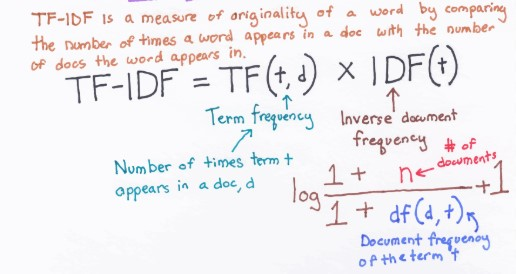
\includegraphics[scale=0.5]{figures/m6.jpg}
		\caption{Lusia-TF IDF}
		\label{contoh}
	\end{figure}
\end{enumerate}






\par
\par
\par
\section{Fadila-1164072}
\subsection{Teori}
Penjelasan Tugas Harian 7 ( No 1-6 )
\begin{enumerate}
\item Pengertian Klasifikasi Teks Dan Ilustrasi Gambar
\begin{itemize}
\item Pengertian Klasifikasi Teks
\par Klasifikasi teks adalah proses pemberian tag atau kategori ke teks sesuai dengan isinya. Teks dapat menjadi sumber informasi yang sangat kaya, tetapi mengekstraksi wawasan darinya bisa sulit dan memakan waktu karena sifatnya yang tidak terstruktur.
\par
\item Ilustrasi Gambar
\par Penjelasan : Berdasarkan pengertian diatas, ada beberapa contoh yang bisa diterapkan. Untuk salah satu contoh dari klasifikasi data sendiri dapat diliat pada gambar berikut \ref{text-fadila}.
\begin{figure}[!hbtp]
\centering
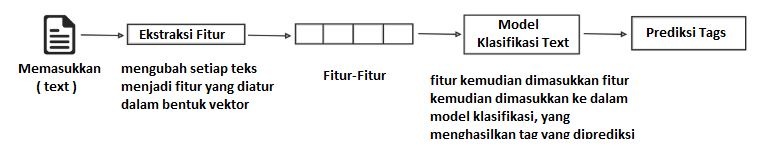
\includegraphics[scale=0.3]{figures/text-fadila.jpg}
\caption{text-fadila}
\label{text-fadila}
\end{figure}
\par
\end{itemize}
\par
\par
\item Mengapa Klasifikasi Bunga Tidak Bisa Menggunakan Machine Learning Dan Ilustrasi Gambar
\begin{itemize}
\item  Mengapa Klasifikasi Bunga Tidak Bisa Menggunakan Machine Learning
\par Penjelasan : Untuk klasifikasi bunga tidak dapat menggunakan machine learning dikarenakan memiliki masalah input yang sama namun keluarannya (output) yang berbeda, biasanya output atau error ini disebut dengan istilah 'noise'. Noise sendiri merupakan output yang disimpan / ditangkap maupun direkam bukan seperti seharusnya ( keluaran yang diiginkan ). 
\par Apabila diberikan contoh, maka contohnya yaitu kita berasumsi secara implisit bahwa klarifikasi bunga yang kita lakukan sudah tepat dan kita melakukannya seperti seorang ahli tanaman. Namun pada hasilnya masih saja terjadi kesalahan. Selain itu, selalu ada peluang untuk memperkenalkan kesalahan saat merekam ataupun menyimpan data, maka harus dilakukan penelitian yang lebih rinci sehingga tidak menimbulkan 'noise' itu sendiri.
\par
\item Ilustrasi Gambar
\par Penjelasan : Berdasarkan pengertian diatas, ada beberapa contoh yang bisa diterapkan. Untuk salah satu contoh dari klasifikasi bunga sendiri dapat diliat pada gambar berikut \ref{bunga-fadila}.
\begin{figure}[!hbtp]
\centering
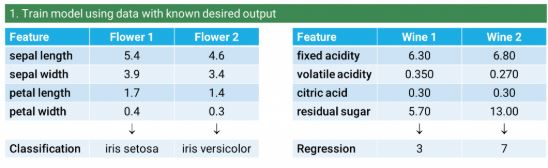
\includegraphics[scale=0.3]{figures/bunga-fadila.jpg}
\caption{bunga-fadila}
\label{bunga-fadila}
\end{figure}
\par
\end{itemize}
\par
\par
\item Teknik Pembelajaran Mesin Pada Teks Pada Kata-Kata Yang Digunakan Di Youtube Dan Ilustrasi Gambar
\begin{itemize}
\item  Teknik Pembelajaran Mesin Pada Teks Pada Kata-Kata Yang Digunakan Youtube
\par Penjelasan : Kita ambil sebuah kasus yang semua orang telah ketahui dan juga pahami. Kasus tersebut yaitu perekomendasian video dari pencarian menggunakan "text / kata" di  Youtube. Pada saat menggunakan Youtube terdapat Machine Learning yang bekerja dan memproses perintah ataupun aktivitas tersebut, dimana akan memfilter secara otomatis video yang disesuaikan dengan "keyword" yang kita masukkan sehingga memberikan keluaran video dengan keyword yang benar. 
\par Adapula fitur yang di dapatkan ketika sedang menonton Youtube. Tampilan sebelah kanan terdapat pilihan 'Next' atapun 'Suggestion' yang menam-
\par pilkan beberapa video serupa sesuai dengan yang dicari atau sedang ditonton. Ketika mengklik salah satu video dari baris tersebut, maka Youtube akan mengingat dan menggunakan kata yang tertera sebagai referensi kembali sehingga akan memberikan kemudahan pada pencarian yang lainnya, Dan disitulah mesin belajar sendiri dan menyimpan data secara berkala sehingga berkembang. 
\par
\item Ilustrasi Gambar
\par Penjelasan : Berdasarkan pengertian diatas, ada beberapa contoh yang bisa diterapkan. Untuk salah satu contoh dari Mesin Teks Youtube sendiri dapat diliat pada gambar berikut \ref{youtube-fadila}.
\begin{figure}[!hbtp]
\centering
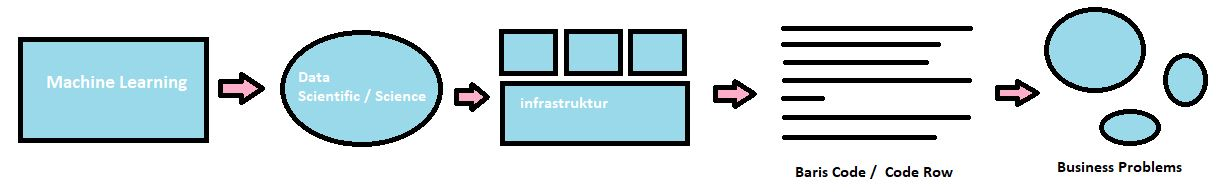
\includegraphics[scale=0.25]{figures/youtube-fadila.jpg}
\caption{youtube-fadila}
\label{youtube-fadila}
\end{figure}
\par
\end{itemize}
\par
\par
\item Vektorisasi Data
\begin{itemize}
\item Maksud Dari Vektorisasi Data
\par Penjelasan : Pembagian dan pemecahan data, kemudian dilakukan perhitungan. Vektorisasi juga dapat dimaksudkan dengan setiap data yang mungkin dipetakan ke integer tertentu. jika kita memiliki array yang cukup besar maka setiap kata / data cocok dengan slot unik dalam array (nilai pada indeks adalah nomor satu kali kata itu muncul).
\par Array angka floating point ( Mewakili data ) :
\begin{itemize}
\item teks
\item audio
\item gambar
\end{itemize}
\par Contoh : -[1.0, 0.0, 1.0, 0.5]
\par
\end{itemize}
\par
\par
\item Pengertian Bag Of Words Dan Ilustrasi Gambar
\begin{itemize}
\item  Pengertian Bag Of Words
\par bag-of-words adalah representasi penyederhanaan yang digunakan dalam pemrosesan bahasa alami dan pengambilan informasi. Model bag-of-words sederhana untuk dipahami dan diterapkan dan telah melihat kesuksesan besar dalam masalah seperti pemodelan bahasa dan klasifikasi dokumen ( penyelesaian dll ).
\par
\par
\item Ilustrasi Gambar
\par Penjelasan : Berdasarkan pengertian diatas, ada beberapa contoh yang bisa diterapkan. Untuk salah satu contoh dari Bag Of Words sendiri dapat diliat pada gambar berikut \ref{bag-fadila}.
\begin{figure}[!hbtp]
\centering
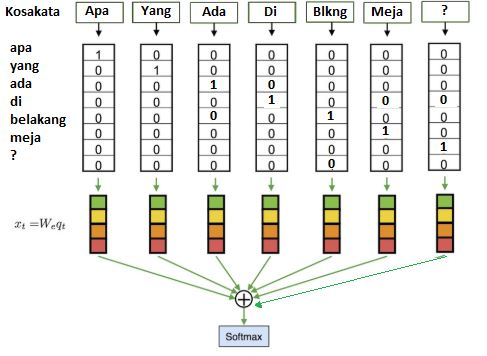
\includegraphics[scale=0.3]{figures/bag-fadila.jpg}
\caption{bag-fadila}
\label{bag-fadila}
\end{figure}
\par
\end{itemize}
\par
\par
\item Pengertian TF-IDF Dan Ilustrasi Gambar
\begin{itemize}
\item  Pengertian TF-IDF
\par TF-IDF atau TFIDF, adalah kependekan dari istilah frekuensi dokumen terbalik, dimana merupakan statistik numerik yang dimaksudkan untuk mencerminkan betapa pentingnya sebuah kata untuk sebuah dokumen dalam kumpulan atau kumpulan.
\par Nilai tf-idf meningkat secara proporsional dengan berapa kali sebuah kata muncul dalam dokumen dan diimbangi dengan jumlah dokumen dalam korpus yang mengandung kata, yang membantu menyesuaikan fakta bahwa beberapa kata muncul lebih sering secara umum
\item Ilustrasi Gambar
\par Penjelasan : Berdasarkan pengertian diatas, ada beberapa contoh yang bisa diterapkan. Untuk salah satu contoh dari TF-IDF sendiri dapat diliat pada gambar-gambar berikut \ref{tf2-fadila}.
\begin{figure}[!hbtp]
\centering
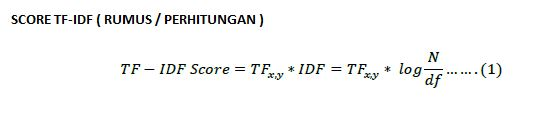
\includegraphics[scale=0.4]{figures/tf2-fadila.jpg}
\caption{tf2-fadila}
\label{tf2-fadila}
\end{figure}
\par
\par
\end{itemize}
\par
\par

\end{enumerate}

\subsection{Praktek}